\RequirePackage[2020-02-02]{latexrelease}
\documentclass{ntuthesis}


\usepackage{amsmath, amssymb}
\usepackage{bm, bbm}
\usepackage{physics}
\usepackage{natbib}

\usepackage{appendix}
\usepackage{caption}    % for subfigure
\usepackage{subcaption} % for subfigure
\usepackage{times}
\usepackage{threeparttablex,longtable}
\usepackage{booktabs}
\usepackage{afterpage}  % load the afterpage package
\usepackage{enumitem}
\usepackage{verbatim}
\usepackage{color}
\usepackage{url}
\usepackage{graphicx}
\usepackage{setspace}
\usepackage{array}
\usepackage{wallpaper}
\usepackage[hidelinks]{hyperref}
\usepackage[printwatermark]{xwatermark}
\usepackage[capposition=top]{floatrow}
\usepackage{chngcntr}
\newcommand{\BL}{\emph{Bitcoin Law}}
\newcommand{\chivo}{\emph{Chivo Wallet}}
\newcommand{\BC}{\emph{Bitcoin City}}

\DeclareMathOperator*{\argmin}{arg\,min}

\newcommand{\refeq}[1]{Equation~({\ref{#1}})}
\newcolumntype{H}{>{\setbox0=\hbox\bgroup}c<{\egroup}@{}}


\counterwithout{equation}{chapter}
\counterwithout{figure}{chapter}
\counterwithout{table}{chapter}
% Using the tex-text mapping for ligatures etc.
\defaultfontfeatures{Mapping=tex-text}
% Set the default fonts
\setmainfont{Times New Roman}
\setCJKmainfont[AutoFakeBold=true,AutoFakeSlant=true]{標楷體}
%\setCJKmainfont[BoldFont={粗楷體},ItalicFont={斜楷體}]{標楷體}

\ifdefined\firstpage

  \def\withwatermark{1}
  \ifdefined\withwatermark
    \newsavebox\mybox
    \savebox\mybox{\tikz[opacity=0.5]\node{
\includegraphics{watermark.pdf}};}
    \newwatermark*[allpages,xpos=6.1725cm,ypos=10.5225cm,scale=0.5]{\usebox\mybox}
  \fi

  % digital object identifier
  \ifdefined\withdoi
    \insertdoi
  \fi
\fi

\makeatletter
\AtBeginDocument{
  \hypersetup{
    pdftitle={\@titleen},
    pdfauthor={\@authoren},
    pdfsubject={\@typeen{} \@classen},
    pdfkeywords={\@keywordsen}
  }
}
\makeatother

% Your information goes here
% author: Tz-Huan Huang [http://www.csie.ntu.edu.tw/~tzhuan]

% ----------------------------------------------------------------------------
% "THE CHOCOLATE-WARE LICENSE":
% Tz-Huan Huang wrote this file. As long as you retain this notice you
% can do whatever you want with this stuff. If we meet some day, and you think
% this stuff is worth it, you can buy me a chocolate in return Tz-Huan Huang
% ----------------------------------------------------------------------------

% Syntax: \var{English}{Chinese}
\university{National Taiwan University}{國立臺灣大學}
\college{College of Social Science}{社會科學院}
\institute{Department of Economics}{經濟學系}
\title{Examining the Chinese Debt-Trap Diplomacy}{檢視中國債務陷阱}
\author{Chia-Wei Chen}{陳家威}
\studentid{R10323045}
\advisor{Tai-kuang Ho, Ph.D.}{何泰寬 博士}
\defenseyear{2023}{112}
\defensemonth{July}{7}
\defenseday{12}
\doi{doi:10.6342/NTU2017XXXXX}
\keywords{Debt-Trap Diplomacy, Belt and Road Initiative, Sovereign Debt, Optimal Default}{債務陷阱外交、一帶一路、主權債務、最適違約決定}


\begin{document}

\frontmatter

\makecover

\ifdefined\excludefirstpage

  \def\withwatermark{1}
  \ifdefined\withwatermark
    \newsavebox\mybox
    \savebox\mybox{\tikz[opacity=0.5]\node{
\includegraphics{watermark.pdf}};}
    \newwatermark*[allpages,xpos=6.1725cm,ypos=10.5225cm,scale=0.5]{\usebox\mybox}
  \fi

  % digital object identifier
  \ifdefined\withdoi
    \insertdoi
  \fi
\fi

% \makecertification

% \begin{acknowledgementszh}
感謝\ldots
\end{acknowledgementszh}

\begin{acknowledgementsen}
I'm glad to thank\ldots 
\end{acknowledgementsen}

% \begin{abstractzh}
關於中國在「一帶一路」倡議下向接受國家提供的過度貸款是否導致這些國家陷入高度債務並最終陷入「債務陷阱」的爭議仍然存在。本論文旨在通過運用一個主權債務模型的校準,從實證角度對這個議題進行考察。具體而言,本研究聚焦於兩個在中國戰略上具有重要地位的國家 --- 斯里蘭卡和巴基斯坦。

研究結果確認了這兩個國家在接受大量貸款後確實陷入了債務違約的狀態。基於這些結果,本研究提出了兩個債務陷阱的類別,並將斯里蘭卡和巴基斯坦分別歸入不同的類別。這種分類方法為債務陷阱外交的相關文獻提供了客觀的評估和呈現方式。
\bigbreak
\noindent \textbf{關鍵字:}{\, \makeatletter \@keywordszh \makeatother}
\end{abstractzh}

\begin{abstracten}

    Ongoing debates remain surrounding whether the excessive loans provided by China under the Belt and Road Initiative lead to high indebtedness and eventual ``debt traps'' for recipient countries. This thesis empirically examines this topic through the calibration of a sovereign debt model. Specifically, the study focuses on two strategically important countries --- Sri Lanka and Pakistan.
    The research findings validate the notion that these two countries indeed fell into the default set once they received substantial loan amounts, allowing for two categories of debt traps into which Sri Lanka and Pakistan reside. This categorization offers an objective assessment and presentation method within the literature on debt-trap diplomacy.
    \bigbreak
\noindent \textbf{Keywords:}{\, \makeatletter \@keywordsen \makeatother}
\end{abstracten}

\begin{comment}
\category{I2.10}{Computing Methodologies}{Artificial Intelligence --
Vision and Scene Understanding} \category{H5.3}{Information
Systems}{Information Interfaces and Presentation (HCI) -- Web-based
Interaction.}

\terms{Design, Human factors, Performance.}

\keywords{Region of interest, Visual attention model, Web-based
games, Benchmarks.}
\end{comment}


% \tableofcontents
% \listoffigures
% \listoftables

\mainmatter


\chapter{Introduction}
As China's economic influence continues to grow, its lending practices to developing countries have come under scrutiny.
The concept of ``debt-trap diplomacy'' (hereinafter DTD), whereby China extends excessive loans to countries in exchange for political or economic concessions, has become a topic of heated debate \citep{Chellaney_2017}.
While some argue that the debt-trap problem poses a significant threat to the economic and political stability of vulnerable countries, others contend that it is overstated.

From the political science aspect, an analysis from the Belfer Center for Science and International Affairs states that China utilizes DTD as a technique to achieve strategic objectives, such as projecting power across South Asian trading routes, undermining regional opposition to its South China Sea claims, and supporting its naval efforts to break out into the Pacific \citep*{Parker2018}.
Critics of this phenomenon argue that claims of DTD are often exaggerated or based on incomplete information. For example, \citet*{Brautigam-meme-2020} argues that the debt-trap is based on a flawed understanding of Chinese lending practices and the histories of the target countries, and that China is not strategically pursuing the DTD on developing countries.

The opacity in Chinese lending practices has been a longstanding challenge in the analysis of the DTD problem \citep*{Horn-Reinhart-Trebesch-21}.
The lack of transparency in the Chinese lending system, whereby loan terms, conditions and collateral requirements are not always disclosed to the borrowers, makes it difficult for economists and policymakers to fully grasp the magnitude of the issue.
Therefore, it has been challenging to assess the sustainability of debts of borrowing countries and their ability to service their obligations, as well as the potential impact of China's lending practices on the economy of low income developing countries (LIDC), especially those in the Belt and Road Initiatives (BLI).
As a result, recent studies on whether DTD is a myth have primarily been conducted normatively in the field of political science, rather than a positive economics analysis~\citep[See, e.g.,][]{Himmer2023-vn,Chen2020-eo}.

However, with the emergence of new and detailed data on Chinese lending practices, recent studies have begun to shed light on the nature and implications of the China debt.
In this thesis, I aim to shed light on whether a country fell into the debt-trap by applying a new and detailed data provided by \citet*{Horn-Reinhart-Trebesch-21}, hereinafter referred to the ``HRT database'', on the sovereign debt model proposed by \citet*{Na-18}, to provide insights into the sustainability of the debt of borrowing countries.
By calibrating the model for a particular country, a set of tradable-output levels which would cause the country to default could be obtained, given its current debt level. Following the approach of \citet{Hinrichsen_2020-chapter4}, this set is presented graphically with each data point on the space representing a debt-output pair for a specific year. This visual representation allows for an examination of whether the country has been in the default zone but has managed to avoid default due to other enforcement mechanisms, in this case might be the political leverage from China.

It requires a lot of work to calibrate all countries to match the model, therefore it is optimal to narrow down the sample countries to those that provides the most insight on the DID issie. I consider countries
\begin{enumerate*}
    \item that is constantly receiving loans from other international institutes,
    \item that indicates an increasing amount of debt from China that eventually exceeds other creditors, and
    \item in which China launches large infrastructure programs.
\end{enumerate*}
% \citet*{Hurley19-8-debt-trap} examines the dept-to-GDP ratio versus the share of China's debt, and identifies eight
% countries\footnote{
%     These countries are Djibouti, Kyrgyzstan, Laos, the Maldives, Mongolia, Montenegro, Pakistan, and Tajikistan}
% that are particularly risky.
In particular, the default sets for Sri Lanka and Pakistan are examined in this thesis. I will further provide the basic backgrounds for the two sample countries in later sections.

\section{HRT Database}
China's official external lending is predominantly undertaken by state-owned entities and the government itself\footnotemark{}. However, unlike other major economies, the Chinese government does not report or publish any data on its official international lending or outstanding overseas debt claims. This lack of transparency creates challenges for rating agencies, as official lending to sovereigns is not a regular part of their activities. Moreover, China is not a member of the Paris Club, which tracks sovereign borrowing from official bilateral creditors, and does not divulge data on its official flows with the OECD's Creditor Reporting System \citep*{Horn-Reinhart-Trebesch-21}.
\footnotetext{These include China's state-owned policy banks, such as China Development Bank (國家開發銀行, CDB) and China Export-Import Bank (中國進出口銀行, Ex-Im), as well as China's state-owned commercial banks such as Industrial and Commercial Bank of China (中國工商銀行, ICBC) or Bank of China (中國銀行, BoC)}

\citet*{Horn-Reinhart-Trebesch-21} combines a variety of sources to construct a consensus database of Chinese official loans.
The HRT database spans from 1949, the establishment of the People's Republic of China, to 2017. It contains a granular dataset of 2151 loans and 2824 grants with information such as the creditor agent, borrower type, commitment, maturity, etc. It also provides an aggregate panel data of the external debt to China for each country.
\begin{figure}[t]
    \centering
    \begin{subfigure}[t]{0.45\textwidth}
        \centering
        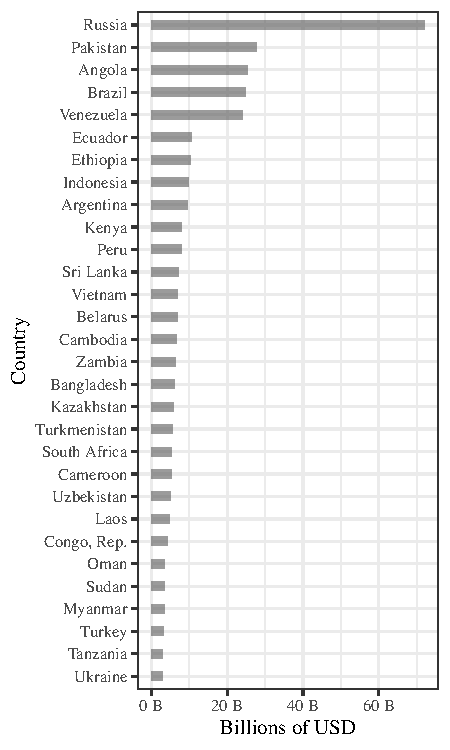
\includegraphics[width = \textwidth]{fig/total_debt.pdf}
        \caption{Top 30 Debtor by Total Debt in USD}
        \label{fig:total-debt-30}
    \end{subfigure}%
    ~
    \begin{subfigure}[t]{0.45\textwidth}
        \centering
        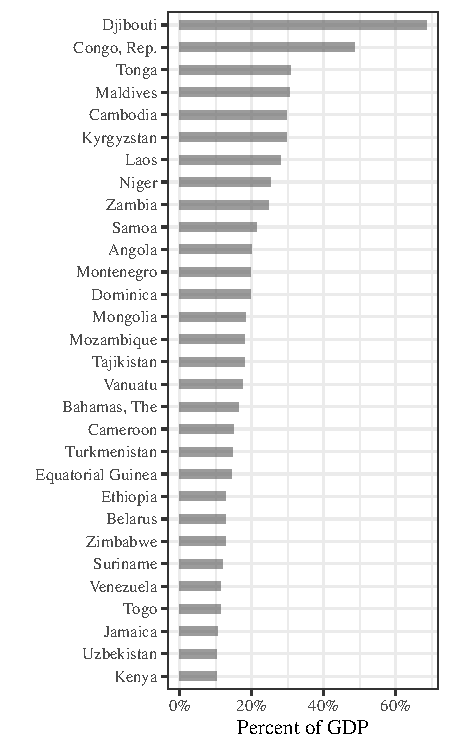
\includegraphics[width = \textwidth]{fig/perc_debt.pdf}
        \caption{Top 30 Debtor by Dept-to-GDP Ratio}
        \label{fig:perc-debt-30}
    \end{subfigure}
    \caption{Debt to China Statistic by Country in 2017}
    \label{fig:Country-Agg}
    \floatfoot{Source: HRT Database \citeyearpar{Horn-Reinhart-Trebesch-21} \\
    Note: The figure on the left presents the top 30 countries in amount of total external debt to China in 2017. The figure on the right compares by the China-debt-to-GDP ratio.}
\end{figure}

The top 30 countries with the largest debts to China's official creditors are displayed in \autoref{fig:total-debt-30}. Notably, Russia owes China over \$70 billion, while Pakistan's debt amounts to \$27 billion, both topping the list. Brazil and Venezuela are among the top 10 countries with the highest debt to China in Latin America. Contrary to what many people believe, African countries have not borrowed much from China. However, if we consider the ratio of Chinese debt to GDP in \autoref{fig:perc-debt-30}, some African countries appear to be highly indebted to China. Djibouti, for instance, has an alarming ratio of 68.5\% of its GDP consisting of Chinese debt, while Tonga, Niger, and Zambia have ratios exceeding 10\%.
\begin{figure}
    \centering
    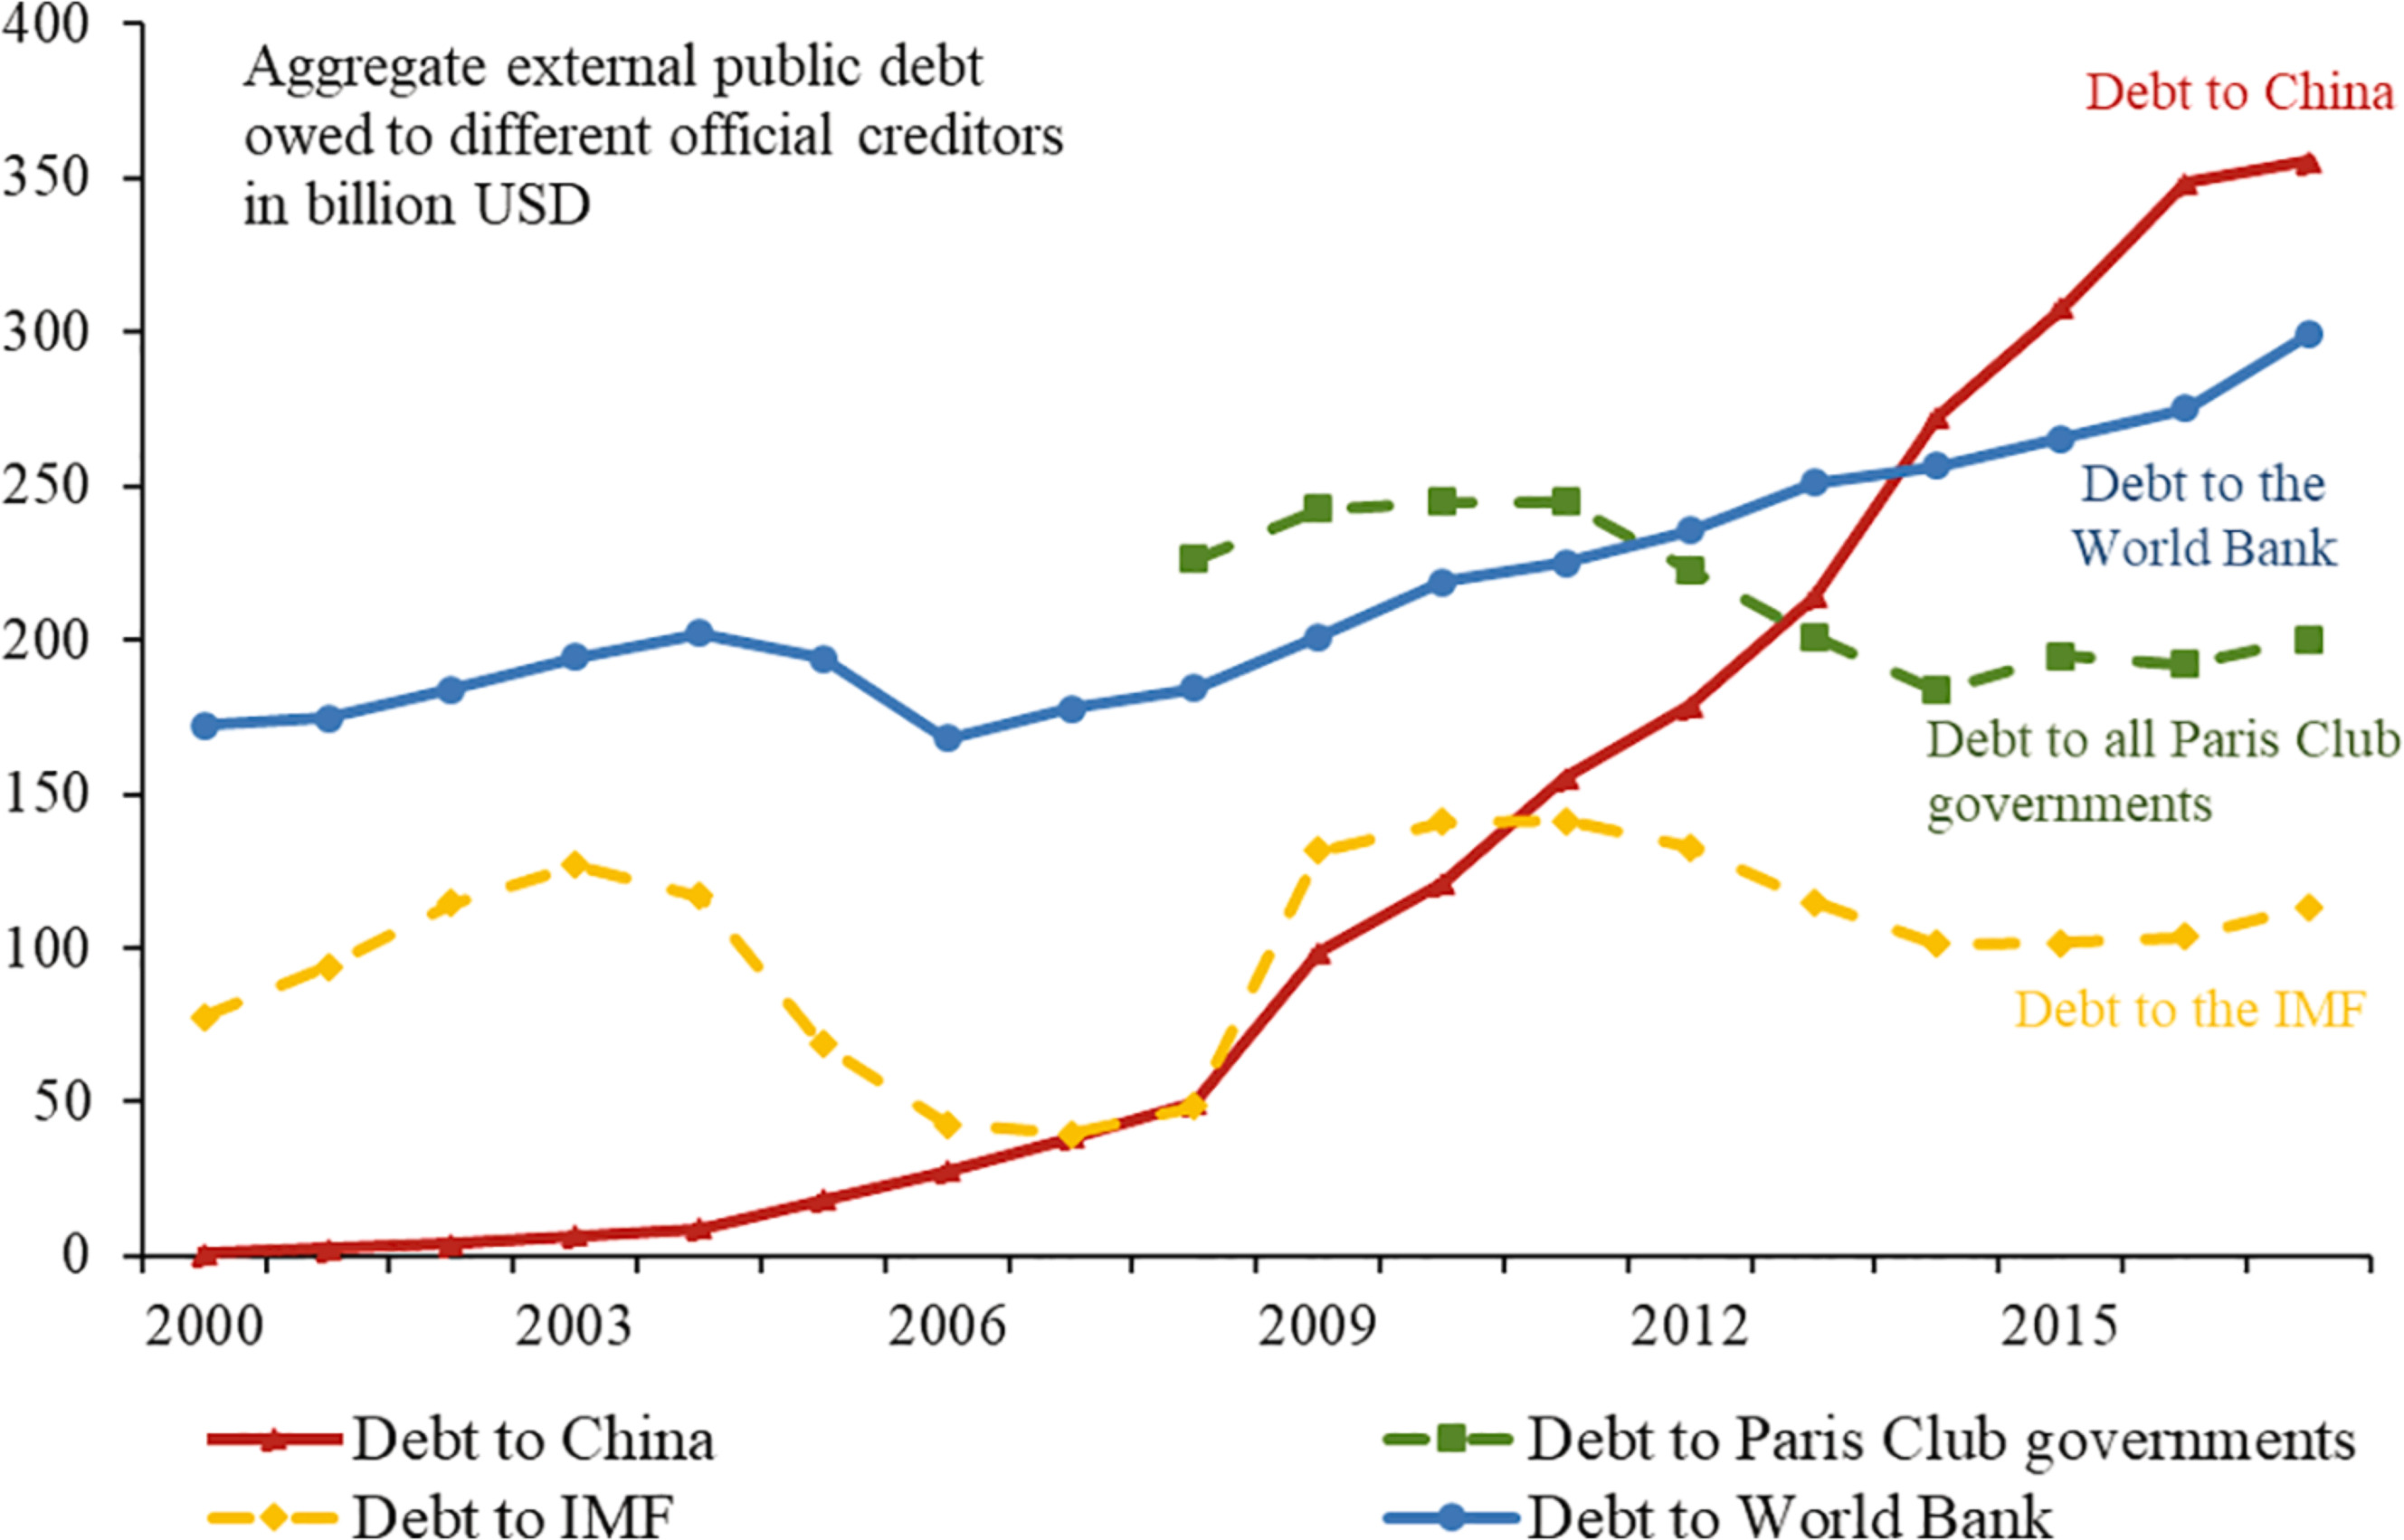
\includegraphics[width = 0.7\textwidth]{fig/temp-external-all-creditor.jpg}
    \caption{Change of Aggregate Public Debt for Different Official Creditors}
    \label{fig:debt-ts}
    \floatfoot{Source: HRT Database \citeyearpar{Horn-Reinhart-Trebesch-21} \\
    Note: The figure shows the change in the aggregate external public debt that the developing countries owed to different official creditors. These include China, World Bank (excluding China), IMF, and all 22 Paris Club governments. It is obvious that China had become the largest official creditors in the world according to the estimation of \citet*{Horn-Reinhart-Trebesch-21}.}
\end{figure}

A main finding in \citet*{Horn-Reinhart-Trebesch-21} is that China had become the world's largest creditor to developing countries after 2013, surpassing the amount of World Bank. \autoref{fig:debt-ts} shows the change of the total amount of debt from different main creditors, including China, World Bank\footnote{Including the International Development Association (IDA) and the International Bank for Reconstruction and Development (IBRD) }, IMF, and the aggregation of all countries in the Paris Club. The debt amount started to rise rapidly after 2000, when the China government launched the ``Go Out Policy'' in 1999. In 2017, the debt to China had reached \$355 billion, while the debt to World Bank was \$300 billion.


This database allows researchers to obtain the true amount of total debt of a country, and gauge the amount of debt that is considered superfluous and onerous for it.
For the next section, I briefly explain the two countries I will examine in my thesis, and demonstrate the importance of choosing it as a benchmark example.

\section*{Sri Lanka}
In the original article where the terminology ``Debt-trap Diplomacy'' was coined, \citet{Chellaney_2017} specifically mentioned the predicament faced by the Sri Lankan government. He argues that the Chinese government supported large infrastructure projects in Sri Lanka and provided heavy loans to their government, and as the project eventually failed to repay the debt, the country is then ensnared in the concessions to China. \autoref{fig: sri-lanka-debt-ts} shows the change in composition of the creditors to Sri Lanka.

The issue of the Hambantota port is regarded as a typical example of a debt-trap for some scholars~\citep*{Moramudali_2020}.
The construction of the port was initiated in 2007 and entrusted to the state-owned Chinese companies --- China Harbour Engineering Company and Sinohydro Corporation. The project was valued at \$361 million, of which Exim Bank financed 85\% at a yearly interest rate of 6.3\%\footnote{From AidData Project ID \#33409, ``China Eximbank provides \$306.7 million buyer's credit loan for Phase I of Hambantota''}.


China's involvement in Sri Lanka's infrastructure development was facilitated by President Mahinda Rajapaksa, during which China became Sri Lanka's leading investor and lender. This gave China significant diplomatic leverage over Sri Lanka. 
However, when Rajapaksa was unexpectedly defeated in the early 2015 election by Maithripala Sirisena, who campaigned on the promise to extricate Sri Lanka from the Chinese debt trap, work on major Chinese projects was suspended.

However, Sri Lanka's government was already on the brink of default, and Sirisena eventually acquiesced to a series of Chinese demands\footnotemark{}, including the sale of an 70\% stake in the Hambantota port to China Merchants Port (CM Port) and a 99-year lease.
\footnotetext{This narrative origins from \citet*{Chellaney_2017}. \citet*{Brautigam-meme-2020}, however, provides a different narrative. She mentioned that ``\emph{The proceeds were used to increase Sri Lanka's
US dollar reserves in 2017-18 with a view to the repayment of maturing international sovereign bonds \dots Therefore, the sale of Hambantota was originally a fire sale designed to raise money to deal
with larger debt problems.}''}
Notably, as argued by \citet*{Moramudali_2019}, the lease did not write off the loans obtained to construct Hambanota port. The proceeds from the lease were used to boost the country's dollar reserves in 2017-18, especially in preparation for the large amount of external debt that needed to be serviced when international sovereign bonds matured in early 2019. This means that the lease is not a debt-equity-swap, as common narratives elaborated \citep*{Moramudali_2020}.
Sri Lanka eventually declared a suspension on payment on most foreign debt from Aril 12, 2022. Whether Sri Lanka was indeed already under the extreme ``brink of default'' during 2015 is a major gap in the literature of sovereign default that has not yet been investigated.

\section*{Pakistan}
Similar to Sri Lanka, we observe the abrupt increase on the debt to China, as it already has a relatively high debt to other official creditors. \autoref{fig: pakistan-debt-ts} shows the change in composition of creditors to Pakistan. 
Pakistan is the centerpiece of the China Pakistan Economic Corridor (CPEC), a 3000 km corridor that connects China with the Arabian sea.
CPEC serves as an important network as it reduces the passage for China's energy import from the Middle Eastern countries \citep*{CPEC-wiki}.

China has launched enormous amounts of infrastructure in Pakistan after 2015. These items include a deep water port, road and rail lines, and most importantly, energy sector projects. Up to 2018, the estimation of the total value of projects under the CPEC is \$62 billion, out of which around \$33 billion is allocated for energy projects~\citep*{Hurley19-8-debt-trap}. China is expected to finance about 80 percent of this amount. The private investments for energy projects in Pakistan will be financed by the Exim Bank of China at an interest rate of 5-6\%. 
Private Independent Power Producers (IPP) will be responsible for constructing the energy projects under CPEC, instead of the governments of China or Pakistan. In turn, the government of Pakistan will be legally bound to buy electricity from these companies at rates that were agreed upon before.
However, despite this significant investment, some projects have already been cancelled, such as three major road projects that were cancelled at the end of 2017 \citep*{Hurley19-8-debt-trap}.

In the case of Pakistan, the sudden increase of debt to China draws the attention of researchers and journalists. For example, a report from the Financial Time titled ``Pakistan is on the brink'' states that Pakistan is following Sri Lanka into default. Given the recent frequent analogy drawn between Pakistan and Sri Lanka, it is essential to analyze Pakistan from the perspective of the sovereign default model.

  \label{ch:intro}
\chapter{Background} \label{ch:background}
  \section{Bitcoin as Legal Tender}\label{sec:bit-el}
  \input{sections/bitcoin.tex}
  \section{FDI in El Salvador}\label{sec:fdi-el}
  \input{sections/FDI-sav.tex}
  
\chapter{Literature Review} \label{ch:lit}
\chapter{Methodology} \label{ch:method}
\input{sections/methodology.tex}
\chapter{Result}  \label{ch:result}
\chapter{Conclusion} \label{ch:conclusion}



\backmatter
\phantomsection
\addcontentsline{toc}{chapter}{\bibname}
\bibliographystyle{apalike}

% Your bibliography goes here
\bibliography{bib/ref.bib}

% \chapter{Appendix}
% \begin{appendices}
%   \section*{The Bitcoin Law}
%   \label{Ap-BitcoinLaw}
%   \input{sections/Append-BitcoinLaw.tex}
% \end{appendices}
\end{document}
